
\section{Running Example}

In order to illustrate the issues with existing notebooks and describe the extensions in \projname\, we will use the following example of a potential analysis:

\begin{example}
Consider a data analyst, working for a news portal website. The analyst would like to create a Jupyter notebook that extracts and presents information about the demographics of the website's reader-base during particular hours. More specifically, the analyst would like to construct a chart showing the number of readers that visit the website during the day; then based on this information, she would like to extract the age groups of the visitors, during different hours of that day and present this to the portal editor. Figure \ref{figure:first-running-example:first-line-chart} shows a sample graph illustrating the number of visitors per hour and Figure \ref{figure:first-running-example:first-bar-chart} shows the age groups of the visitors. By doing this, the analyst can convince the portal editor to publish more articles and advertisements that target particular age groups during hours in which they visit the portal the most, thus maximizing the portal's revenue and reader's satisfaction.
\end{example}

\begin{figure}[ht]
  \centering
  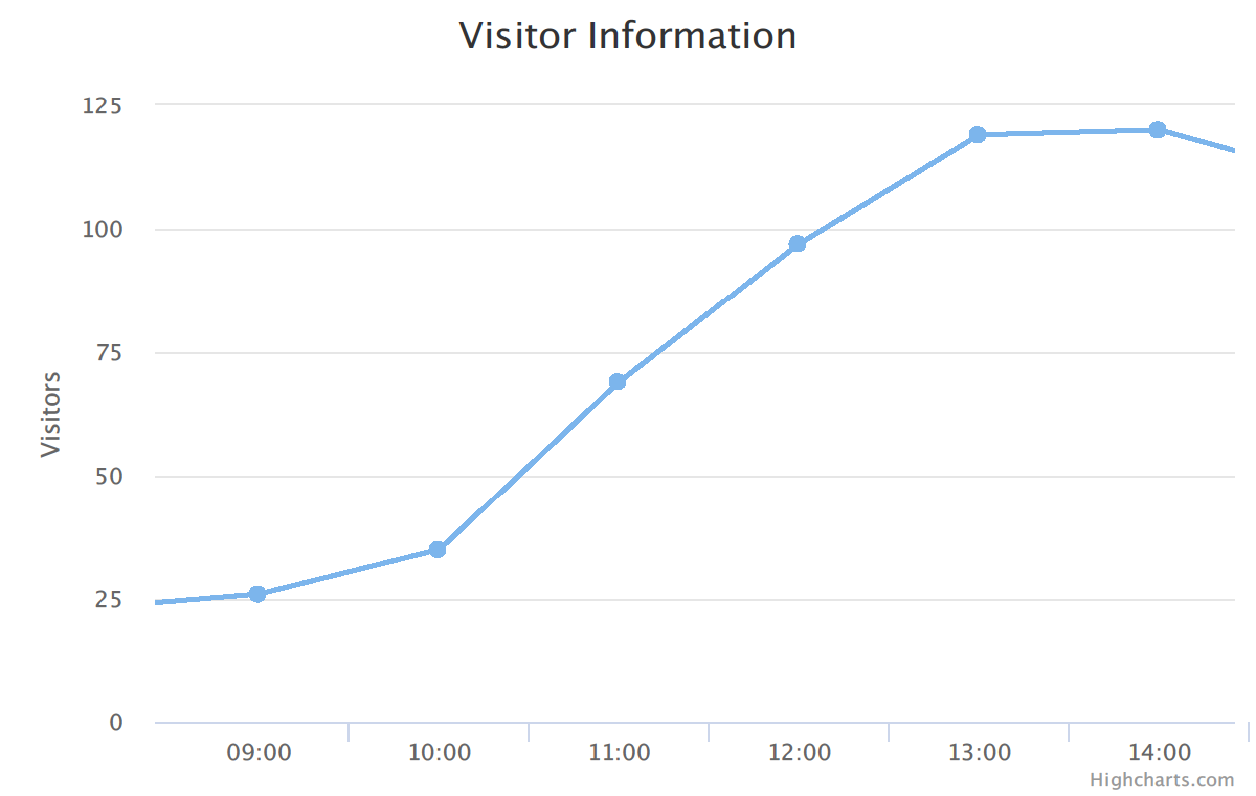
\includegraphics[width=0.8\columnwidth]{figures/first-line.png}
  \caption{Line chart showing visitors per hour}
\label{figure:first-running-example:first-line-chart}
  %\vspace*{\floatsep}% http://tex.stackexchange.com/q/26521/5764
   \vspace*{0.1cm}
  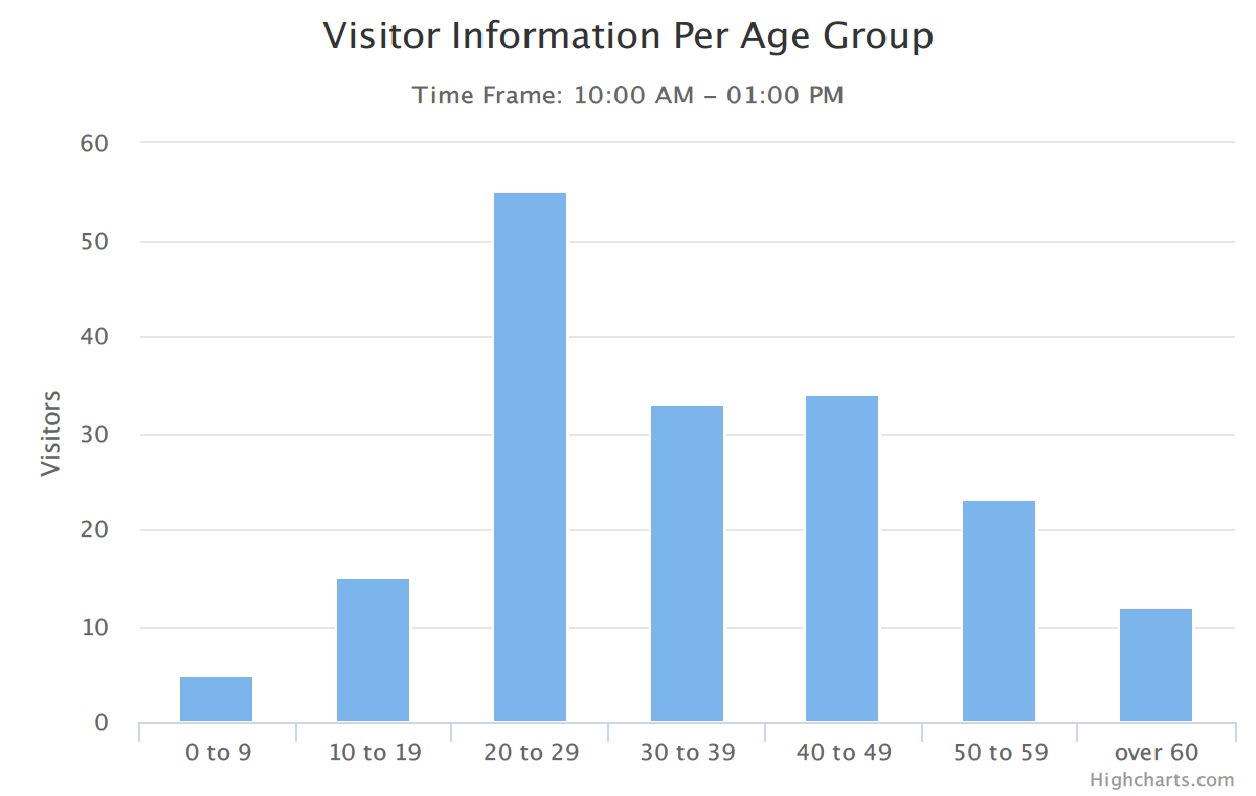
\includegraphics[width=0.8\columnwidth]{figures/first-bar.png}
  \caption{Bar chart showing age groups of visitors}
  \label{figure:first-running-example:first-bar-chart}
\end{figure}



For this analysis, we assume that the news portal maintains information about its reader-base in a database system. Table \ref{tab:schema} shows a potential database schema, that could be used for storing visitor information. The database contains two tables, namely ``Page Views" and ``Visitors"; table ``Visitors" contains information about each reader, such as the reader id, name, lastname, username and age. The table ``Page Views" maintains a tuple for each visit, and it consists of a visit id, the visitor id (foreign key referencing the visitor), and the time in which the user visited the website. The reader information could have been retrieved, with their permission, from various social media services (such as Facebook, Google etc). In order to construct this notebook, the data analyst must (a) retrieve  website access information from the database, by joining the two tables on the visitor id (b) generate a plot that shows the number of users that visit the website during the day, (c) issue a query that counts the number of visitors per age group, for each potential set of selected hours, and (d) create a bar chart that shows the number of visitors per age group. 


\subsection{Issues with Traditional Notebooks}



We will now describe the steps required for performing this analysis in a traditional interactive notebook that uses Python. While we do so, we will describe the issues that arise.

\noindent {\bf Setting up and interacting  with third-party utility libraries - Security concerns.} Before even starting working on any of the afore-mentioned tasks the data analyst must make sure that all third-party python packages that will be used for retrieving and visualizing data, are installed. This step will either introduce a dependency between the analyst and some system administrator, or the analyst will need the appropriate access rights in order to perform the installation, typically, using a command line. The latter can be a security concern (especially, if the server on which the notebook operates, also hosts other applications) or can lead to corrupted systems if not performed correctly. The complexity of this step increases as the number of utility libraries, our analyst wants to use, increases. \eat{More specifically, for cases when an analyst needs to access data stored in a MongoDB and a MySQL database, two drivers will need to be installed.}

\begin{table}
\begin{center}

\begin{tabular}{|c|c|c|c|}
\hline 
\multicolumn{4}{|c|}{Page Views} \\ 
\hline 
id & vid & url & time \\ 
\hline 
\end{tabular} 

\hfill

\begin{tabular}{|c|c|c|c|c|}
\hline 
\multicolumn{5}{|c|}{Visitors} \\ 
\hline 
vid & name & lastname & username & age \\ 
\hline 
\end{tabular} 

\end{center}
\caption{Schema description of the two tables in our database.}
\label{tab:schema}
\end{table}


Once the system is configured, the analyst needs to read lengthy documentation pages in order to properly issue queries to the employed database system, using the API of the respective library. This step typically requires the use of imperative code that interacts with the library. During this step, the analyst has to also specify the credentials that will be used for accessing the database system. In most such libraries, the credentials have to be inlined into the method call that establishes the connection with that system. While this would not be a security concern in a python application (since the code that includes the credentials would have been compiled into a binary file, thus hiding the credentials), in a python notebook, the credentials would lie in plain sight for anyone, who has access to the notebook, to see.

\noindent {\bf Data model conversions.}
After, establishing the connection with the database system, and issuing the queries, the analyst, is able to consume the results by using the internal, to the library, datamodel. After doing so, the analyst has to again read documentation pages in order to infer the data model dictated by the visualization library she selected, and manually perform the appropriate conversions in order to construct the first visualization, by invoking the appropriate renderer function. Note that data model conversions have to take place every time the analyst wishes to integrate a third-party library in her analysis, so the amount of ``plumbing code" required, can quickly skyrocket.


\noindent {\bf Limited interactive exploratory capabilities.}
The next step, is for the analyst to issue a query that counts the visitors per age group for a set of selected hours and construct a bar chart showing the result. Note, however, that there's no straightforward way for selecting a meaningful range of hours. The analyst will have to go through a process of trial and error, by issuing an arbitrary number of such queries and plotting the results, until she finds a set that produces valuable insight. Furthermore, even if the analyst goes through this process for the data corresponding to a particular day, the hour range selection she made, might not produce any valuable insight for the dataset corresponding to another day. 

\noindent {\bf Discussion about reactive charts.} The use of co-dependent reactive charts could have been proven useful in this scenario. If the analyst was able to use a chart that allows the reader to select a particular range of hours by using the first plot, she could use that input in order to retrieve and plot only the user demographics for this particular range. Figure \ref{fig:reactive-data-processing} graphically depicts this process. The first figure shows the reader of the notebook, selecting a particular time frame. this causes the line chart to zoom in showing only the selected time frame. After the update, the subsequent bar chart is also updated thus only showing the age groups of the visitors in the selected time frame. This feature would add useful exploratory capabilities, to the notebook, which would be of great value to notebook readers. It would enable them to further analyze the underlying dataset without writing any lines of code. 

It is important to note that this feature cannot be implemented currently in interactive notebooks. Instead, the analyst would have to implement a full blown application in order to enable users interact with visualizations in this way. This requires more time and effort as well as technical expertise with web frameworks that data analysts, might lack. This reactive behavior requires the implementation of actions that have to be invoked when particular mouse events take place on the pixels of the browser that correspond to the visualization. Additionally, such events have to take place in a specific order (mousedown-mousemove-mouseup). The developer of such applications must install observers that listen for such events and then provide the application logic that asynchronously accesses a back-end database in order to retrieve new data based on the user's selection and then cause the appropriate mutations to the respective visualizations that depend on that data.
\begin{figure}[]
\centering
	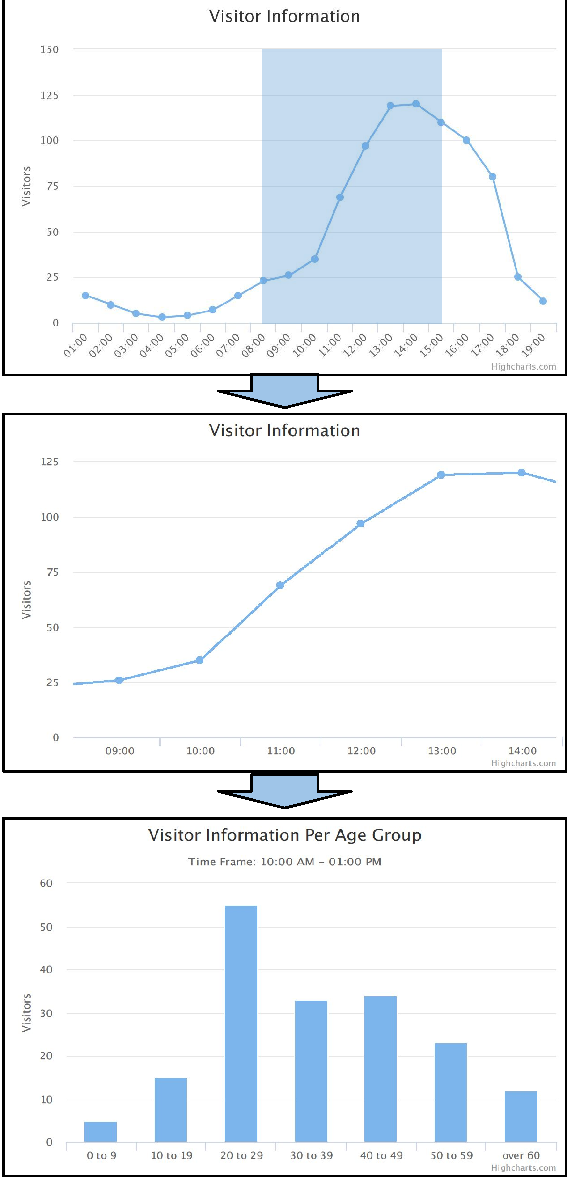
\includegraphics[width=0.7\columnwidth]{figures/reactive-processing.pdf}
	\caption{Demonstration of reactive charts. The reader's selection automatically updates both charts.}
	\label{fig:reactive-data-processing}
\end{figure}

 

\subsection{Simplifying and Enhancing Interactive Notebooks}

In this section we will describe how the \projname\ notebook engine deals with the aforementioned challenges. Firstly, \projname\ notebooks support two types of modules that shield analysts from low level coding, namely: \textbf{source wrappers} and \textbf{visual units}. Source wrappers allow the use of source specific languages for querying database systems (for instance SQL can be used to query MySQL and PostgreSQL databases). When using source wrappers, data analysts directly provide a query on the notebook interface and receive the result in JSON format. Visual units are constructs that input JSON and generate visualizations. Both source wrappers and visual units come pre-installed and can be used by data analysts without the installation of any additional packages. Additionally, since no method calls are required for accessing and visualizing data, the analyst does not have to read long documentation files before using them. 

In order for source wrappers to connect to the respective database systems, the data analyst must provide a configuration file, describing the information required for establishing a connection with each source. Such configuration files are added by interacting directly with the notebook interface, therefore data analysts do not have to use a command line during setup. Once added, these files are hidden from the UI and encrypted thus diminishing any security concerns. Lastly, visual units are constructs that take as input JSON objects (in a predefined format) and generate visualizations on the notebook interface. 


Source wrappers produce and visual units consume JSON. Since both these constructs use the JSON data model, no data model transformations are required by the analyst. This minimizes the amount of plumbing code required for generating an analysis. For cases when the data analyst wishes to perform some additional computation or perform data transformations, \projname\ also supports a declarative template language that operates on JSON data. This template language also allows the invocation of functions. Regardless of whether these functions are defined by users or by third-party packages they must operate on the JSON data model, in order to be used in a template.

This language also allows data analysts tp describe reactive behavior. Specifically, by binding individual variables to certain parts of the visual unit, data analysts can collect information which can later be used in other parts of the notebook. By doing so, analysts can describe computation that depends on the reader's input. \projname's propagation algorithm, identifies statements that depend on such libraries and triggers their evaluation. This process leads to truly interactive notebooks, that react to the reader's input, thus enhancing the exploratory capabilities of traditional notebooks.

\eat{
Source wrappers require the instantiation of a configuration file, that describes the information required for establishing a connection with each source. Such configuration files are added by data analysts by interacting directly with the notebook interface. Once added, these files are hidden from the UI and encrypted thus diminishing any security concerns. Lastly, visual units are constructs that take as input JSON objects (in a predefined format) and generate visualizations on the notebook interface. 


Most importantly, source wrappers and visual units, both use the same data model JSON, so no data model transformations are required for retrieving and visualizing data. For cases when the data analyst wishes to perform some data transformations, \projname\ also supports a declarative template language.


Once a source wrapper receives a query, it propagates it to the respective database system, and then parses and returns the result in JSON format. Source wrappers require the instantiation of a configuration file, that describes the information required for establishing a connection with each source. Such configuration files are added by data analysts by interacting directly with the notebook interface. Once added, these files are hidden from the UI and encrypted thus diminishing any security concerns. Lastly, visual units are constructs that take as input JSON objects (in a predefined format) and generate visualizations on the notebook interface. 

Both source wrappers and visual units come pre-installed and can be used directly on the notebook without the installation of any additional packages. Additionally, since no method calls are required for accessing and visualizing data, the analyst does not have to read long documentation files before using them. Most importantly, source wrappers and visual units, both use the same data model JSON, so no data model transformations are required for retrieving and visualizing data. For cases when the data analyst wishes to perform some data transformations, \projname\ also supports a declarative template language.
}

\eat{
interactive chart implementation using imperative languages is not a trivial task and possibly beyond the coding skill set of an average data analyst. Such a task requires advanced coding skills and implementation of event listeners to capture the user's mouse input and asynchronously trigger execution of other functions that will update data and re-draw the second figure. As we show later in Section ??, the {\projname} framework is equipped with modules that can take care of the heavy work, while the analyst only needs to define ``bound'' (linked) variables.


Finally, 


plot a line chart of access count Vs timestamp, as well as a bar chart of access count Vs age groups, and (c) be able to select a time range from the line chart using mouse input and automatically filter and display data in the second plot to present age-group-based activity within the selected time frame. 


The data analyst can access historic data about the user base by directly querying the data base system. Table \ref{tab:schema} shows the database schema. The analyst's first task is to retrieve the data via database queries, join the two tables based on the visitor id (``vid'') key and group by (1) ``time'' and (2) ``age'' to prepare the data for the two plots.

Installing packages, transferring data and connecting with database systems requires technical knowledge that often exceeds the skill-set of a typical data scientist. Lastly, while such notebooks support the generation of visualizations with the use of the appropriate library



Throughout this paper, we present {\projname} via an example data analysis: We assume a scenario where a data analyst must (a) retrieve  website access information from a database, (b) plot a line chart of access count Vs timestamp, as well as a bar chart of access count Vs age groups, and (c) be able to select a time range from the line chart using mouse input and automatically filter and display data in the second plot to present age-group-based activity within the selected time frame. 

For our walkthrough example, we assume a Jupyter server where the analysts develop their notebooks and a different database server where data is stored. Table \ref{tab:schema} shows how our databases are organized. The analyst's first task is to retrieve the data via database queries, join the two tables based on the visitor id (``vid'') key and group by (1) ``time'' and (2) ``age'' to prepare the data for the two plots.

During the visualization stage, the analyst implements two ``linked'' plots in such a way that a range selection in the first plot \textit{automatically} (without re-executing code in the notebook) filters the data presented in the second plot. Figure \ref{fig:vision} illustrates the expected chart behavior. A time-frame selection in the first chart (10:00AM - 1:00PM) causes the second chart to only plot those accesses that occurred during the selected interval. 

It is important to note that this interactive chart implementation using imperative languages is not a trivial task and possibly beyond the coding skill set of an average data analyst. Such a task requires advanced coding skills and implementation of event listeners to capture the user's mouse input and asynchronously trigger execution of other functions that will update data and re-draw the second figure. As we show later in Section ??, the {\projname} framework is equipped with modules that can take care of the heavy work, while the analyst only needs to define ``bound'' (linked) variables.
}
